\begin{tikzpicture}
    \tkzDefPoint(0,0){A} % Define el primer punto
    \tkzDefPoint(4,0){B} % Define el segundo punto
    \tkzDefPoint(6,2){C} % Define el tercer punto
    \tkzDefPoint(2,2){D} % Define el cuarto punto

    \tkzDrawPolygon(A,B,C,D) % Dibuja el paralelogramo

    % Dibuja los ángulos marcados
    \tkzMarkAngle[size=0.8](B,A,D)
    \tkzLabelAngle[pos=0.5](B,A,D){$\alpha$}
    
    \tkzMarkAngle[size=0.8](D,C,B)
    \tkzLabelAngle[pos=0.5](D,C,B){$\alpha$}
    
    \tkzMarkAngle[size=0.4](A,D,C)
    \tkzLabelAngle[pos=0.2](A,D,C){$\beta$}
    
    \tkzMarkAngle[size=0.4](C,B,A)
    \tkzLabelAngle[pos=0.2](C,B,A){$\beta$}

    % Etiqueta los puntos
    \tkzLabelPoints[below](A,B)
    \tkzLabelPoints[above](C,D)
\end{tikzpicture}